\section{Marken \& Produkte}
\subsection{Manner}
\piccaption[Logo Manner\cite{josef_manner_marken}]{Logo Manner\cite{josef_manner_marken}}
\parpic[r]{
\includegraphics[scale=0.5]{images/logo_manner.png}}
\enquote{\enquote{Chocolade für alle – preiswert und gut}, das war die Devise von Josef Manner I. bei der Gründung der Süßwarendynastie im Jahre 1890. Dieser Grundsatz gilt auch heute für die zahlreichen Köstlichkeiten der Marke Manner.\\\\
Erfahren Sie mehr, von den im Hause Manner gerösteten Kakaobohnen bis zu köstlichen Produktneuheiten... stets dem Motto \enquote{Manner mag man eben} folgend!
}\cite{josef_manner_marken}
\picskip{0}

\subsection{Casali}
\piccaption[Logo Casali\cite{josef_manner_marken}]{Logo Casali\cite{josef_manner_marken}}
\parpic[r]{
\includegraphics[scale=0.5]{images/logo_casali.png}}
\enquote{Die Geschichte der Firma Casali reicht weit zurück in die Vergangenheit. Im Jahr 1782 gründete Joseph Casali in der damals zur k. u. k. Monarchie gehörenden Hafenstadt Triest seine Firma. Seit 1970 ist Casali, bekannt für köstliche Rum-Kokos Kugeln und fruchtige Schoko-Bananen, Teil der Josef Manner \& Comp. AG.}\cite{josef_manner_marken}
\picskip{0}

\subsection{Victor Schmidt}
\piccaption[Logo Victor Schmidt\cite{josef_manner_marken}]{Logo Victor Schmidt\cite{josef_manner_marken}}
\parpic[r]{
\includegraphics[scale=0.5]{images/logo_victorschmidt.png}}
\enquote{Die weltberühmten Mozartkugel erweist nicht nur Wolfgang Amadeus Mozart die Ehre. Sie wurde im Laufe der Jahrzehnte ähnlich der Manner Schnitte ein Synonym für österreichische Süßwarentradition - eng verbunden mit österreichischer Hochkultur.\\\\
Lernen Sie die feinen Besonderheiten der unvergleichlichen Victor Schmidt Austria Mozartkugel kennen! LiebhaberInnen feinsten Marzipans, zarten Nougats und knackiger Bitterschokolade werden begeistert sein...}\cite{josef_manner_marken}
\picskip{0}

\subsection{Ildefonso}
\piccaption[Logo Ildefonso\cite{josef_manner_marken}]{Logo Ildefonso\cite{josef_manner_marken}}
\parpic[r]{
\includegraphics[scale=0.5]{images/logo_ildefonso.png}}
\enquote{Die Geschichte von Ildefonso ist nicht nur eine süße, sondern auch eine interessante. Sie begann gegen Ende des 19. Jahrhunderts. Im Jahr 1880 entwickelte ein Konfektmeister von Victor Schmidt die feine Rezeptur des beliebten Schicht-Nougatwürfels. Mit 1. Jänner 2000 wurde die Firma Victor Schmidt \& Söhne von Manner erworben.\\\\
Lernen Sie die vielschichtigen Seiten des beliebten Wiener Nougat-Konfekts kennen.}\cite{josef_manner_marken}
\picskip{0}
\newpage
\subsection{\#winak}
\piccaption[Logo \#winak\cite{josef_manner_marken}]{Logo \#winak\cite{josef_manner_marken}}
\parpic[r]{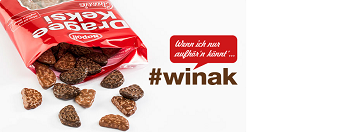
\includegraphics[scale=0.5]{images/logo_winak.png}}
\enquote{Dragee Keksi von Napoli spielen eine besondere Rolle im Napoli Produktsortiment. Daher haben sie einen eigenen Online Auftritt, der diesem österreichischen Keks-Klassiker in unterhaltsamer Art und Weise gerecht wird.
Lernen Sie das Motto der Dragee Keksi \enquote{wenn ich nur aufhör`n könnt`} persönlich kennen. Unter dem Hashtag \#winak sorgen Dragee Keksi für eine nicht enden wollende Portion Spaß im digitalen Alltag!}\cite{josef_manner_marken}
\picskip{0}

\subsection{Napoli}
\piccaption[Logo Napoli\cite{josef_manner_marken}]{Logo Napoli\cite{josef_manner_marken}}
\parpic[r]{
\includegraphics[scale=0.5]{images/logo_napoli.png}}
\enquote{Unter der Marke Napoli bieten wir hochwertige Produkte für besonders preisbewußte KonsumentInnen an. Abseits der Dragee Keksi von Napoli umfasst das Sortiment vorwiegend Waffelprodukte, wie beispielsweise den Napoli Schnittenblock. Einen eigenen Online-Auftritt haben die Napoli Produkte derzeit nicht.}\cite{josef_manner_marken}
\picskip{0}
